\documentclass{article}

%Margins
\usepackage[margin=1in]{geometry}


%Float & Graphics 
\usepackage{float}
\usepackage{graphicx}

%Chemistry Equations
\usepackage [version = 3] {mhchem}

%Document
\begin{document}
\begin{titlepage}
\title{Solubility of \ce{C_{12}H_{22}O_{11}_{(s)}} and \ce{NaCl_{(s)}} in 50 mL of \ce{H_2O_{(l)}} at $25^o C$ and $100^o C$ in 1 ATM}
\author{Abhishek Sreekanth}
\date{1-8-2014}
\maketitle
\thispagestyle{empty}
\end{titlepage}
\setcounter{page}{1}

%Sections 
\section*{Abstract}
The purpose of this experiment was to determine the solubility of sucrose and sodium chloride. Sucrose had the greatest solubility, both in overall solubility and average differences in solubility. The sucrose had a greater solubility due to its bond type: Polar-covalent. Sucrose has the same bond type as water, therefore, has the greatest solubility. The results of this experiment supported the claim that if a solvent and the solute has a polar-covalent bond, then it will have the greatest solubility. 
\pagebreak
\section*{Introduction} %Introduction
\subsection*{Purpose} %Purpose
The purpose of this experiment was to determine the solubility of Sucrose and Sodium Chloride, by adding the solutes into water, until even after vigorous and prolonged stirring, the solute remained undissolved. 
\subsection*{Background} %Background
For the purposes of this experiment, only two types of bonds will be discussed: ionic and polar-covalent. Ionic bonds, generally, occur between metals and nonmetals; furthermore, between atoms with low and high electronegativity's. Polar-covalent bonds occur between two non-metals and generally occur with atoms of varying electronegativity's. These two types cause compounds to have certain, very different, properties. \\\\
%Properties of Ionic compounds
Ionic compounds have high melting and boiling points as the molecules are arranged in a crystal lattice. Most ionic compounds, in the solid state, form crystals. Ionic compounds do conduct electricity, only if the ions in the compound are free to move; therefore, ionic compounds conduct electricity only when they are dissolved in water or melted. If an ionic compound is soluble in water, a salt forms when the compound reacts with an alkali in an acid reaction (Tro, 2001) . \\\\
%Properties of Polar-covalent Compounds 
Polar-covalent compounds have low melting points- relative to ionic compounds. Polar-covalent compounds, however, have higher melting points than non-polar covalent bonds. They are generally poor electrical conductors- in all phases. Polar-covalent compounds are only soluble in other polar compounds, such as water (Tro, 2007). \\\\
%Solubility Preamble 
The solubility of a substance is the amount of a substance that will dissolve in a given amount of solvent. Many factors effect solubility, but intermolecular forces either promote or prevent the formation of a solution. A solution either forms, or does not form, depending on the types of intermolecular forces present in both solute and solvent. Entropy, energy dispersed in a system, is also a factor in deterring if two substances form a solution. The greater the entropy, the more likely a solution will be formed (Tro, 2007). \\\\
The following table illustrates the conditions in which a solution will either form or not form:\\
%Chart showing when a solution forms or not 
\begin{figure}[H]
	\centering
	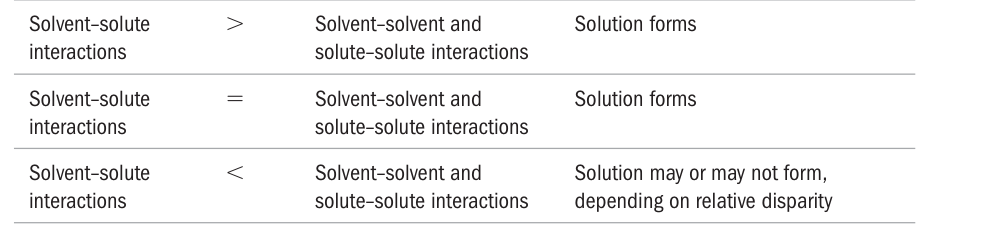
\includegraphics{lr21.png} 
\end{figure} 
%Miscibility
Two substances are said to be miscible if they are soluble in each other in all proportions. In general, similar substances form solutions and dissimilar solutions do not. For example, polar solvents dissolve many polar ionic solutes, and non-polar solvents dissolve non-polar solutes. If two substances are dissimilar they may still form a solution, if and only if, the disparities are diminutive, if they are too large then they will not form a solution (Tro, 2007)
%Sodium Chloride preamble 
\begin{figure}[H]
	\centering 
	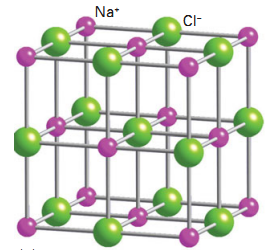
\includegraphics{ncl.png}
	\caption{Three-dimensional molecular structure of Sodium Chloride}
\end{figure}
%Description 
\ce{NaCl_{(s)}}, commonly referred to as table salt, is an ionic crystalline compound with a 1:1 ratio of Sodium ions and Chloride ions. \ce{NaCl} is bounded in a cubic lattice, as depicted above.The substance is a small, solid, colorless crystal. \ce{NaCl} has a boiling point of $1465^o C$ and a melting point of $800.7^o C$. \ce{NaCl} has a theoretical solubility of $\frac{36.0g \ce{NaCl}}{100.0mL \ce{H_2O}}$ at $25^o C$ (Pubchem.gov). \\\\
%Sucrose Preamble 
\begin{figure}[H]
	\centering
	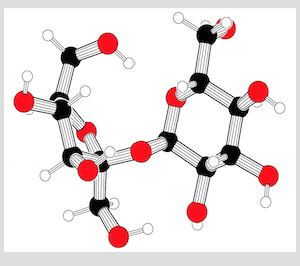
\includegraphics{s22.png}
	\caption{Three-dimensional structure of Sucrose}
\end{figure} 

\begin{figure}[H]
	\centering
	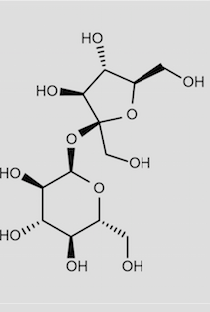
\includegraphics{s11.png}
	\caption{Lewis Structure of Sucrose}
	\end{figure}
%Discussion 
\ce{C_{12}H_{22}O_{11}_{(s)}}, commonly referred to as sugar or sugar, is a polar covalent compound with a 6:11:5.5 ratio of  carbon, hydrogen, and oxygen ions. \ce{C_{12}H_{22}O_{11}_{{(s)}}} is a white powdery solid. \ce{C_12H_{22}O_1{(s)}} has a melting point of $185.5^o C$. \ce{C_{12}H_{22}O_{11}_{{{(s)}}}} has a theoretical solubility of $\frac{45g \ce{C_{12}H_{22}O_{11}}}{50.0mL \ce{H_2O}}$ at $25^O C$ (Pubchem.gov). \\\\


%Previous Studies, justification, dependent and independent variables  
A previous study was conducted on the solubility of Fluorite in hydrothermal solutions. In this study Fluorite was dissolved in various hydrothermal solvents. The solubilities were determined by using temperature, bond-types, and various other physical properties of the solvent. All of these solutions were tested at temperatures below $300^o C$. The experiment determined that only a handful of complexes had the properties necessary to play a major role in fluorite transport at temperatures below $300^o C$ (Richardson, Holland, 1979).\\\\
%Justification of This Experiment 
This experiment was conducted to understand how solutes and solvents behave when dissolving. This basic knowledge can then be applied to the large scale to produce commercial products. Using these basic principles and the knowledge obtained from this experiment, the results can be transferred and applied to many more commercial purposes and pharmaceuticals. The experimental variable is the solubility and the independent variable is the temperature of the solvent.  
\subsection*{Hypothesis} %Hypothesis 
If Sucrose and Sodium Chloride are dissolved in water then Sucrose will have a greater solubility because it is a polar-covalent solute dissolving in a polar-covalent solvent. \\\\
\subsection*{Safety Information} %Safety Information 
Safety is paramount, and good laboratory practices should not only be informed, but also practiced. The risk of burn was apparent, all throughout the experiment. Simple measures must be taken to prevent any sort of burn injuries. The hot-plates used, and hot beakers should be stationed at an area, away from foot traffic. Proper equipment should be used to touch and move the hot equipment, and lastly, safety googles must be worn at all times, in case of splattering. 

\section*{Materials}
\begin{enumerate}
\item 50 mL Burette	(1) \\
\item 250 mL Beaker (1)\\
\item 140 mL Beaker	(2) \\
\item Burette stand (1) \\ 
\item Hot Plate	 (1) \\
\item	Timer (1) \\ 
\item	Stirring rod  (1) \\
\item	Thermometer (1) \\
\item	Tong (1) \\
\item	Paper (1) \\
\item	Pencil (1) \\
\item Weighing Dish (1) \\
\item	Scale (1) \\
\item	650mL \ce{H_2O} (apx.) \\
\item	120g  \ce{NaCl_{s}} (apx.) \\
\item 600g  \ce{C_{12}H_{22}O_{11}_{s}} (apx.)
\end{enumerate}

\section*{Procedure}
%Sodium and Sugar room temp. 
Sodium Chloride was weighed in a weighing dish on an electronic scale. 50 mL of water was poured through a burette into a 140 mL beaker. A temperature probe was then inserted into the beaker to measure the temperature of the water. A soon as the probe read $25^o C$  Sodium Chloride was slowly poured into the beaker. While the salt was slowly poured into the solution, the resulting solution was being vigorously stirred. As soon as a small amount of salt stuck to the bottom of the beaker, no more salt was poured. The solution was stirred vigorously for 30 seconds. If the salt had not dissolved, the remaining Sodium Chloride in the weighing dish was subtracted from the initial value, and the ratios were calculated. This experiment was repeated 2 additional times .\\\\
%Sugar room temp
For Sucrose, only 25 mL of water was poured through a burette into a 140 mL beaker.  A temperature probe was then inserted into the beaker to measure the temperature of the water. A soon as the probe read $25^o C$  Glucose was slowly poured into the beaker. While the sugar was slowly poured into the solution, the resulting solution was being vigorously stirred. As soon as a small amount of sugar stuck to the bottom of the beaker, no more sugar was poured. The solution was stirred vigorously for 30 seconds. If the sugar had not dissolved, the remaining Glucose in the weighing dish was subtracted from the initial value, and the ratios were calculated. The final ratios were then multiplied by two. This process was repeated 2 more times.  \\\\
%Sodium and sugar boiling  
A boiling plate was initially heated, while the boiling plate was heating, 50 mL of water was poured through a burette into a 140 mL beaker. A temperature probe was inserted into the beaker and the beaker was placed on top of the heating plate. The temperature was carefully monitored, as soon as the probe read $100^o C$ the beaker was immediately removed from the hot plate onto a flat lab-table surface. The Sodium Chloride was then slowly poured into the beaker until a minuscule amount stuck to the bottom. The solution was then stirred for 30 seconds and if the salt still failed to dissolve, the remaining amount of Sodium Chloride in the weighing dish was subtracted from the initial amount and the results were calculated. This experiment was repeated 2 additional times. 
%Sugar Boiling 
For Sucrose, only 25 mL of water was poured through a burette into a 140mL beaker.  A temperature probe was inserted into the beaker and the beaker was placed on top of the heating plate. The temperature was carefully monitored, as soon as the probe read $100^o C$ the beaker was immediately removed from the hot plate onto a flat lab-table surface. The Glucose was then slowly poured into the beaker until a minuscule amount stuck to the bottom. The solution was then stirred for 30 seconds and if the sugar still failed to dissolve, the remaining amount of Glucose in the weighing dish was subtracted from the initial amount and the results were calculated. This experiment was repeated 2 additional times and the final solubilities were multiplied by two. 
 \section*{Results}
 \subsection*{Raw Data}
%Sodium Room tempt table 
\begin{table}[H]
	\centering 
	\small
	\title{Solubility of \ce{NaCl_{(s)}} in \ce{H_2O_{(l)}} at $25^o C$} 
	\tabcolsep=0.11cm 
	\begin{tabular}{ccccc} \\
	Trail No. & Initial Weight $(\pm .001)$ (g) & Final Weight $(\pm .001)$ (g) & Amount Dissolved $(\pm .00017)$ ($\frac{g}{50mL \ce{H_2O}}$) & Solubility $(\pm .00017)$ ($\frac{g}{mL}$) \\ \hline \\
		1 & 49.942 & 31.594 & $\frac{18.348}{50}$ & .36696 \\\\ 
		2 & 49.938 & 30.947 & $\frac{18.991}{50}$ & .37982 \\\\ 
		3 & 50.015 & 31.085 & $\frac{18.930}{50}$ & .37860 \\\\
	\end{tabular}
	\caption{Data and resulting calculations for \ce{NaCl} at $25^o C$} 
	\end{table} 


%Glucose (room temp.) Table
\begin{table}[H]
	\centering
	\small
	\title{Solubility of \ce{C_{12}H_{22}O_{11}_{(s)}} in \ce{H_2O_{(l)}} at $25^o C$}
	\tabcolsep=0.11cm 
	\begin{tabular}{ccccc} \\
	Trail No. & Initial Weight $(\pm .001)$ (g) & Final Weight $(\pm .001)$ (g) & Amount Dissolved $(\pm .0004)$ ($\frac{g}{25mL \ce{H_2O}}$) & Solubility $(\pm .0004)$ ($\frac{g}{mL}$) \\ \hline \\
	1 & 55.698 & 3.756 & $\frac{51.942}{25}$ & 2.07768 \\\\
	2 & 56.726 & 4.694 & $\frac{51.066}{25}$ & 2.04264 \\\\
	3 & 55.786 & 4.382 & $\frac{51.404}{25}$ & 2.05616 \\\\
	\end{tabular}
	\caption{Data and resulting calculations for \ce{C_{12}H_{22}O_{11}} at $25^o C$} 
	\end{table}


%Sodium (hundred deg.) Table
\begin{table}[H]
	\centering
	\small 
	\title{Solubility of \ce{NaCl_{(s)}} in \ce{H_2O_{(l)}} at $100^o C$} 
	\tabcolsep=0.11cm 
	\begin{tabular}{ccccc} \\
	Trail No. & Initial Weight $(\pm .001)$ (g) & Final Weight $(\pm .001)$ (g) & Amount Dissolved $(\pm .00017)$  ($\frac{g}{50mL \ce{H_2O}}$) & Solubility $(\pm .00017)$  ($\frac{g}{mL}$) \\ \hline \\
	1 & 55.256 & 36.002 & $\frac{19.254}{50}$ & 0.38508 \\\\
	2 & 54.876 & 35.345 & $\frac{19.531}{50}$ & 0.39062  \\\\
	3 & 55.815 & 36.163 & $\frac{19.652}{50}$ & 0.39304 \\\\
	\end{tabular}
	\caption{Data and resulting calculations for \ce{NaCl_{(s)}} at $100^o C$} 
	\end{table}


%Glucose (hundred deg.) Table 
\begin{table}[H]
	\centering
	\small
	\title{Solubility of \ce{C_{12}H_{22}O_{11}_{(s)}} in \ce{H_2O_{(l)}} at $100^o C$}
	\tabcolsep=0.11cm 
	\begin{tabular}{ccccc} \\
	Trail No. & Initial Weight $(\pm .001)$ (g) & Final Weight $(\pm .001)$ (g) & Amount Dissolved $(\pm .004)$ ($\frac{g}{25mL \ce{H_2O}}$) & Solubility $(\pm .004)$ ($\frac{g}{mL}$) \\ \hline \\
	1 & 125.859 & 4.114 & $\frac{121.745}{25}$ & 4.86980 \\\\
	2 & 124.974 & 2.875 & $\frac{122.099}{25}$ & 4.88396 \\\\
	3 & 123.847 & 2.545 & $\frac{121.032}{25}$ & 4.84128 \\\\
	\end{tabular}
	\caption{Data and resulting calculations for \ce{C_{12}H_{22}O_{11}} at $100^o C$} 
	\end{table}
\begin{figure}[H]
	\centering
	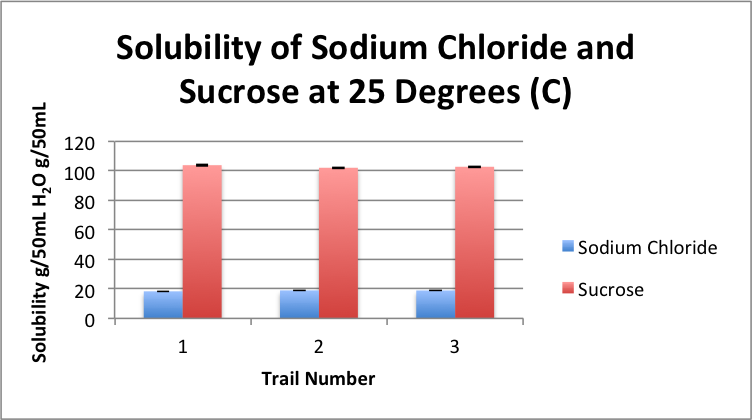
\includegraphics{g1.png}
	\caption{Solubility of Sodium Chloride vs Sucrose at $25^O C$}
\end{figure}
\begin{figure}[H]
	\centering
	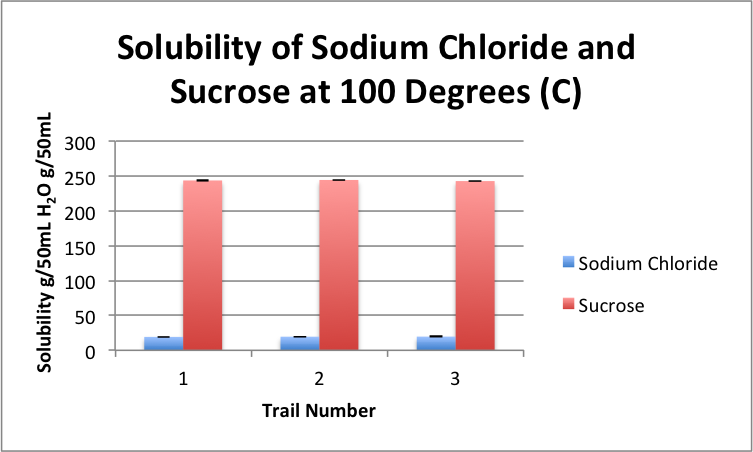
\includegraphics{g2.png}
	\caption{Solubility of Sodium Chloride vs Sucrose at $100^o C$}
\end{figure}
\subsection*{Important Results}
Sucrose had a higher solubility than Sodium Chloride at both $25^o C$ and $100^o C$. On average Sodium Chloride had a solubility of .581 $(\pm .07)$ $\frac{g}{mL}$ at $25^o C$ and an average solubility of .592 $(\pm .07)$ $\frac{g}{mL}$. Sucrose, however, had an average solubility of 2.059 $(\pm .07)$ $\frac{g}{mL}$ at $25^o C$ and an average solubility of 4.865  $(\pm .07)$ $\frac{g}{mL}$ at $100^o C$
\subsection*{Calculations}
The only calculations used in this experiment was for determining the uncertainties for the Solubility ratios. Relative uncertainties had to be calculated to determine  the proper error. \\\\
%Sucrosee
Uncertainty for Sucrose:
$\frac{Uncertainty of Sucrose}{Mass of Sucrose} = Relative Uncertainty of Sucrose$ \\\\
$\frac{Uncertainty of Water}{Volume of Water} = Relative Uncertainty of Water$ \\\\
$Uncertainty of Solubility = (Uncertainty of Sucrose + Uncertainty of Water)Solubility$ \\\\
Calculations:
\begin{eqnarray}
\frac{.001}{121.745} &=& 7.9 x 10^-6 \\
\frac{.02}{25} &=& 8.0x10^-4 \\
Uncertainty of Solubility &=& 8.0x10^-4  +  7.9x10^-6 \\
(4.0 x10^-4+7.9 x 10^-6 )4.8698 &=& .004 \\
\end{eqnarray}

This same process is repeated for the other trials and for Sodium Chloride.


\section*{Discussion} 
\subsection*{Results and hypothesis}
The hypothesis states that Sucrose would have a greater solubility in water than Sodium Chloride, because Sucrose and Water have the same bond type. The results support the hypothesis. In all 3 trails and both water temperatures. Figure 4 help's visualize the differences in solubilities. Sucrose's Solubility is significantly larger than that of sodium during all 3 trails. That difference only becomes greater at $100^o C$, as depicted by Figure 5. The differences within the two substances also differs greatly. On average, the solubility Sodium Chloride had a difference of .011 $(\pm .00034)$ $\frac{g}{mL}$. Sucrose, however, had an average difference in solubility of 2.806 $(\pm .008)$ $\frac{g}{mL}$. The polar-covalent bonds of Sucrose not only caused the solubility of Sucrose to increase, but also caused the increase in temperature of solvent to have a greater effect on its solubility. \\\\
In conclusion, this experiment supports the hypothesis and the claim that bond-type does effect solubility. And that a polar-covalent solute dissolved in a polar-covalent solvent will yield a solution with the greatest solubility. \\
\subsection*{Experimental Error}
This experiment was associated with errors, like all experiments. First, no measuring device is perfectly precise, and carry a certain uncertainty value. Second, $100^o C$ is the boiling point of water. This is the temperature at which water boils, therefore, some of the water could have evaporated causing the solubility to be slightly incorrect. Third, the method used to measure the solubility had a lot of errors associated with it as well. Some extra solute could have fallen out while pouring it into the water and caused the solubility ratios to become greater than they really are. Lastly, the stirring might not have been consistent enough or vigorous enough to determine if the solution was fully saturated or not. This could have caused the solubility to become less than it actually is. These results help answer the research question, how will the two solubilities of substances differ depending on the solute and the solvent's bond types, because the results for both trails show that the Sucrose had the greater solubility. Both Figure 4 and Figure 5 show the extent to which the solubilities vary, and the bonds between Sodium Chloride and Water differ, whereas, Sucrose and Water have the same bond types: Polar Covalent. Thus supporting the hypothesis and answering the research question: The solute with the same bond type as the solvent will have the greatest solubility. \\
\subsection*{Improvements}
To reduce the listed errors, alternate methods should be used. The most precise lab materials should be used, to reduce all the listed errors. The beaker with the boiling water should be covered to prevent any water from evaporating. An alternate method could have been used to measure the solubility more precisely, measuring the amount of solute left after vaporization, but the solution could have been stirred with an automatic stirrer all throughout the experiment and the solute should have been slowly funneled into the already stirring solution. This way the stirring would be uniform and consistent, there wouldn't be any variations during each trail. Lastly, there could have been more trails run to collect more data and to more accurately determine the solubility. 
\end{document}